\subsection{Experimental Setup}
\paragraph{Compared Methods}
\begin{figure}[h]
    \centering
    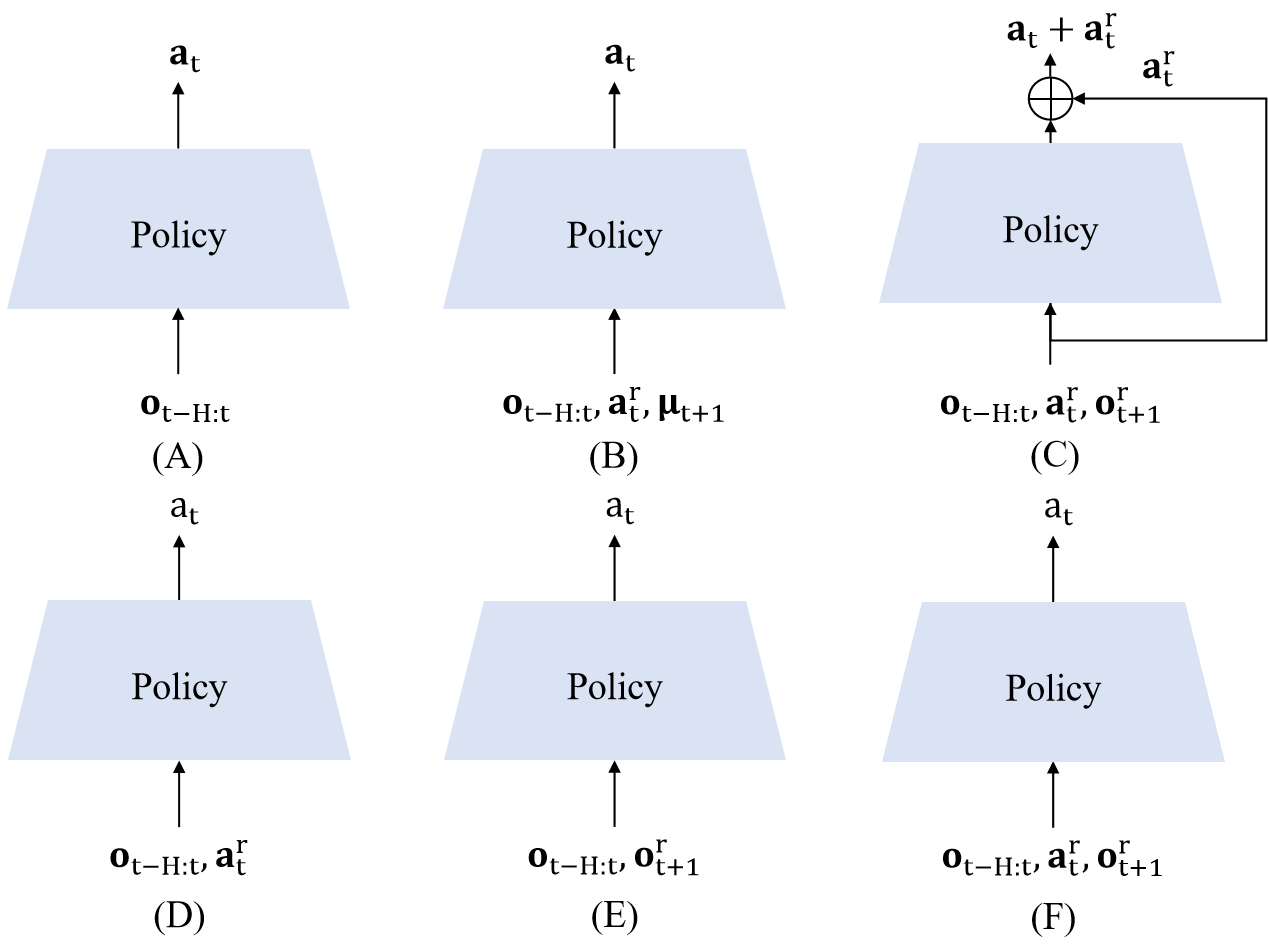
\includegraphics[width=1\linewidth]{fig/baseline.png}
    \caption{Compared Methods.}
    \label{fig:baseline}
\end{figure}

To fairly compare our method with others, we set up five variants as Figure~\ref{fig:baseline}.

(A) Baseline: Train with current and history observations, equivalent here to~\cite{long2024him};
(B) Ours w/o Adjust: Ours without observation reference adjustment, the mean value output from the dynamics model is used directly as the observation reference;
(C) Ours w Residual: Action reference is summed with the actor output as action output, similar to residual policy in~\cite{silver2018residual, yuan2024policy};
(D) Ours w/o Action Reference: Action reference input is set to zero tensor;
(E) Ours w/o State Reference: State reference input is set to zero tensor;
(F) Ours;

\paragraph{Simulation Setup} We use the PPO algorithm with 4096 parallel environments and a rollout length of 100 time steps in Isaac Gym~\cite{rudin2022learning}. The training process takes 4096 parallel environments for 2000 iterations in the NVIDIA A800 GPU. In Section \ref{sec5_2_2}, we trained longer iterations to observe learning curves.

\subsection{Evaluation on Simulator}
\subsubsection{Command Tracking}
We evaluate the tracking errors in linear velocity and angular velocity per second for each algorithm under various terrains.
Tracking errors are calculated by
${\|v_{x,y} - v_{x,y}^{\text{target}}\|^2}$ and ${\|\omega_{\text{yaw}} - \omega_{\text{yaw}}^{\text{target}}\|^2}$ 
respectively.
The results in Table~\ref{tab:tracking_error} show that our method has a lower velocity tracking error.

\begin{table}[thb]
%\footnotesize
    \centering
    \caption{Average Tracking Error in Simulator over 1000 Trials.}
    \label{tab:tracking_error}
    \scalebox{1.2}{
    \begin{tabular}{llllll}
        \hline
        \makecell[l]{Terrain Types} & \makecell[l]{Velocity Types} & Baseline & Ours \\
        \hline
        \multirow{2}{*}{\makecell[l]{Smooth Slopes}} 
        & Linear & 0.170 & \textbf{0.120} \\
        & Angular & 0.101 & \textbf{0.099} \\
        \hline
        \multirow{2}{*}{\makecell[l]{Rough Slopes}} 
        & Linear & 0.387 & \textbf{0.162} \\
        & Angular & 0.164 & \textbf{0.130} \\
        \hline
        \multirow{2}{*}{\makecell[l]{Stairs}} 
        & Linear & 2.371 & \textbf{0.992} \\
        & Angular & \textbf{0.515} & 0.552 \\
        \hline
        \multirow{2}{*}{\makecell[l]{Discrete}} 
        & Linear & 1.955 & \textbf{0.120} \\
        & Angular & 0.220 & \textbf{0.099} \\
        \hline
    \end{tabular}
    }
    \vspace{-0.2in}
\end{table}

\subsubsection{Learning Curve}
\label{sec5_2_2}
\begin{figure}[h]
    \centering
    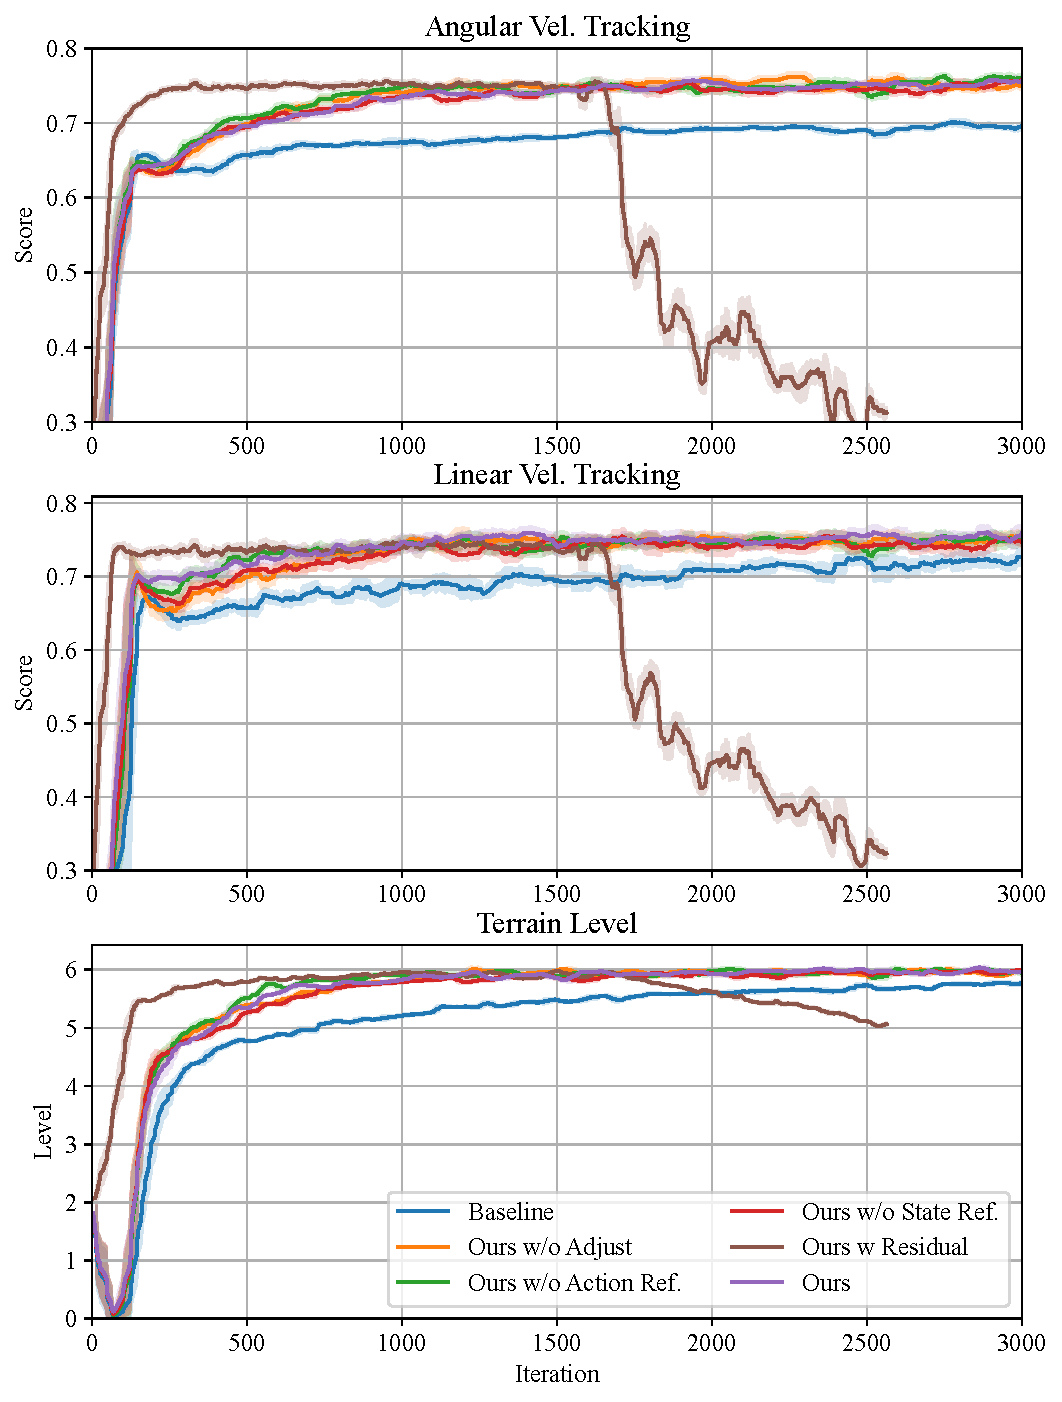
\includegraphics[width=1\linewidth]{fig/curve.pdf}
    \caption{\textbf{Ablation studies with learning curves.} From top to bottom: (1) normalized linear velocity tracking score, (2) normalized angular velocity tracking score, and (3) maximum reachable terrain level in training.}
    \label{fig:curve}
\end{figure}
We recorded the growth of velocity tracking score and terrain passing ability for different algorithms during training.
The normalized angular velocity tracking score and the normalized linear velocity tracking score are calculated by $\text{exp}(-\frac{\|\omega_{\text{yaw}} - \omega_{\text{yaw}}^{\text{target}}\|^2}{0.25})$ 
and $\text{exp}(-\frac{\|v_{x,y} - v_{x,y}^{\text{target}}\|^2}{0.25})$
respectively.
The terrain is categorized into 9 difficulty levels based on the curriculum setting, the same as~\cite{long2024him}.

Observing from the learning curves in Figure~\ref{fig:curve}, our method consistently maintains an advantage over the baseline in terms of tracking error and terrain traversal ability throughout the training process.
Notably, after the introduction of action residual, the method crashed in the middle of training. Based on previous analysis, there is a distribution shift between reference learning and policy learning. 
Although residual concatenation of reference action of imagined transitions improves the speed of policy learning early in training, the imagined transitions are unreliable when encountering the OOD state, leading to potential policy training breakdowns.
Our adjustment mechanism of the dynamics model aims to mitigate the adverse effects of this OOD issue.

\subsubsection{Payload Shift}
\begin{figure}[h]
    \centering
    \includegraphics[width=1\linewidth]{fig/payload-min.pdf}
    \caption{\textbf{Success rate of different algorithms under various payloads.} The success rate for payloads from 1kg to 9kg on both smooth and rough slopes is 100\%.}
    \label{fig:payload}
\end{figure}

\begin{figure*}[htb]
    \centering
    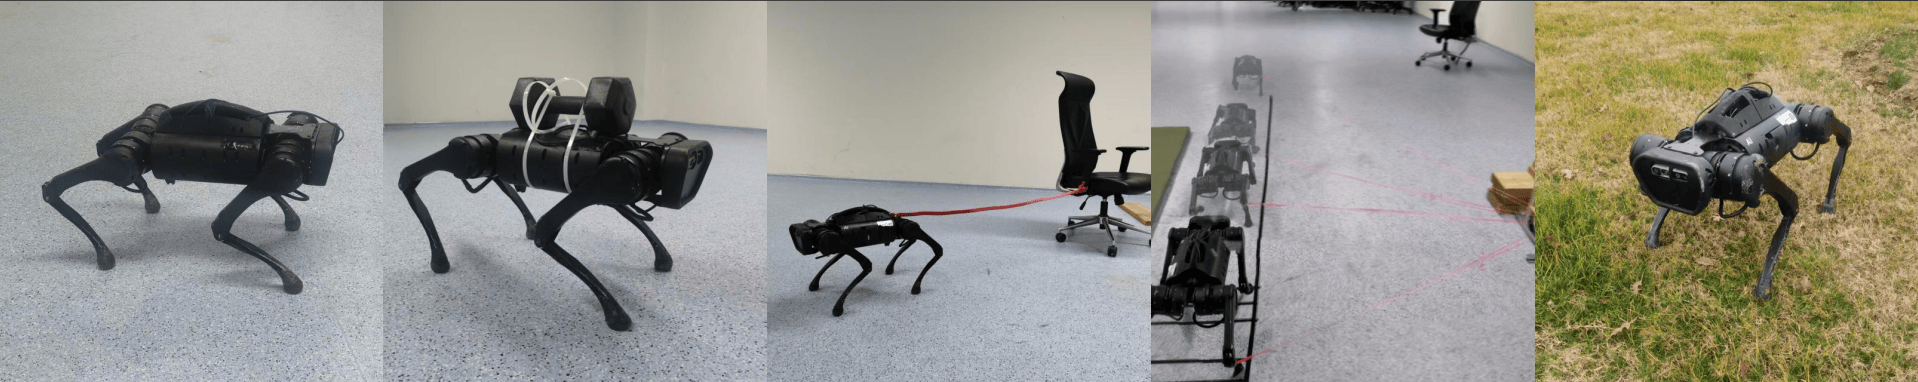
\includegraphics[width=1\linewidth]{fig/realworld.png}
    \caption{\textbf{Deployment on Real World.} Five scenarios in order from left to right: (1) Plane - flat surface walking, (2) Payload - carrying 3 Kg additional weight, (3) Disturbance-1 - external force applied from the back, (4) Disturbance-2 - external disturbance applied to the right-back leg, and (5) Lawn - walking on uneven grassy terrain.}
    \label{fig:realworld}
\end{figure*}

To verify the performance of our approach against the unknown heavy payload, we tested the success rate of the A1 robot in executing different payloads on four different terrains: smooth slopes, rough slopes, stairs up, and stairs down with varying levels of difficulty. 
The robot was required to walk forward with the command [1, 0, 0](m/s) in all four terrains for 200 steps. The range of payload gradually increases from 1kg to 20kg. For smooth and rough slopes, we execute 100 times with different seeds, and since the terrain of stairs is more complicated, we execute 1000 times to calculate the success rate, and the result is shown in Figure~\ref{fig:payload}.

On all test terrains, our method survived significantly better than the other compared methods when faced with unseen heavy loads.
In addition, we can find that although the changes in state adjustment and action reference input do not show significant differences in the learning curve and the evaluation within the distribution, they affect the performance of the method in unseen payloads.

\subsubsection{Adding push to robots}
\begin{figure}[h]
    \centering
    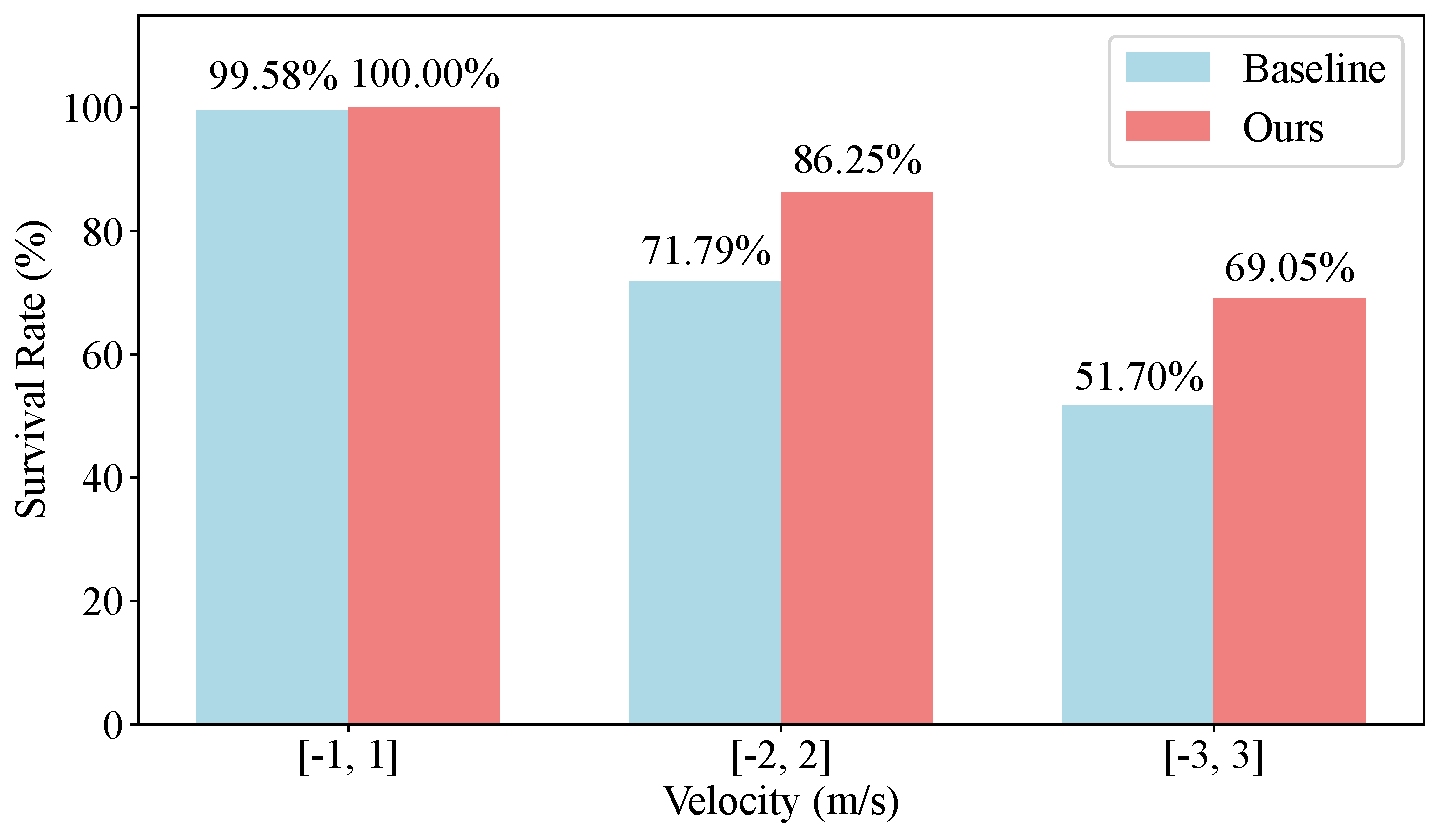
\includegraphics[width=1\linewidth]{fig/push_bar.pdf}
    \caption{\textbf{Comparison of survival rate under external pushing.} The experimental results are categorized into three classes based on the magnitude of the external push velocity. A higher survival rate indicates better robustness.}
    \label{fig:push_bar}
\end{figure}

Pushing a robot with external force is a widely used method for evaluating the robustness of its locomotion. 
In this experiment, the push force was applied by adding a random velocity to the quadruped’s base along the \(xy\)-plane of the world frame. 
The robot was instructed to walk forward with a command of \([1, 0, 0] \, \text{m/s}\), while simultaneously responding to the unpredicted random push. 
The magnitude of the added velocity determines the intensity of the push, with larger magnitudes corresponding to more forceful pushes. 
To assess the robustness of our approach in comparison to the baseline, pushes were randomly sampled 2000 times within a velocity range of \([-3, 3] \, \text{m/s}\). 
The results in Figure~\ref{fig:push_bar} illustrate that our method outperforms the baseline in terms of fall resistance when subjected to external pushes.

% \begin{table}[h]
% %\footnotesize
% \tabcolsep=2pt
%     \centering
%     \caption{Survive Rate under Pushing at Different Velocities.(\%(survives/total))}
%     \label{tab:vel_success_rate}
%     \scalebox{1.2}{
%     \begin{tabular}{cccc}
%         \hline
%         Velocity (m/s) & Baseline &
%         Ours & Improvement(\%) \\
%         \hline
%         $[-1, 1]$ & \makecell[c]{99.58\\(237/238)} & \makecell[c]{100\\(238/238)} & 0.42 $\uparrow$ \\
%         $[-2, 2]$ & \makecell[c]{71.79\\(616/858)} & \makecell[c]{86.25\\(740/858)} & 14.46 $\uparrow$ \\
%         $[-3, 3]$ & \makecell[c]{51.70\\(1034/2000)} & \makecell[c]{69.05\\(1381/2000)} & 17.35 $\uparrow$ \\
%         \hline
%     \end{tabular}
%     }
% \end{table}

Figure~\ref{fig:push} provides a detailed visualization of the standing versus falling status under various push magnitudes and directions for different algorithms.
Given the command \([1, 0, 0] \, \text{m/s}\), it can be observed that Figure~\ref{fig:push} exhibits near-symmetry along the \(x\)-axis, but not along the \(y\)-axis. All methods include push perturbations within the range \([-1, 1] \, \text{m/s}\) during the robust training phase, and consequently, they perform well within this range. However, as the perturbation range increases, the advantage of our approach becomes increasingly pronounced. Our method outperforms the baseline by surviving more than 300 additional times in 2000 randomized tests.

\begin{figure}[h]
    \centering
    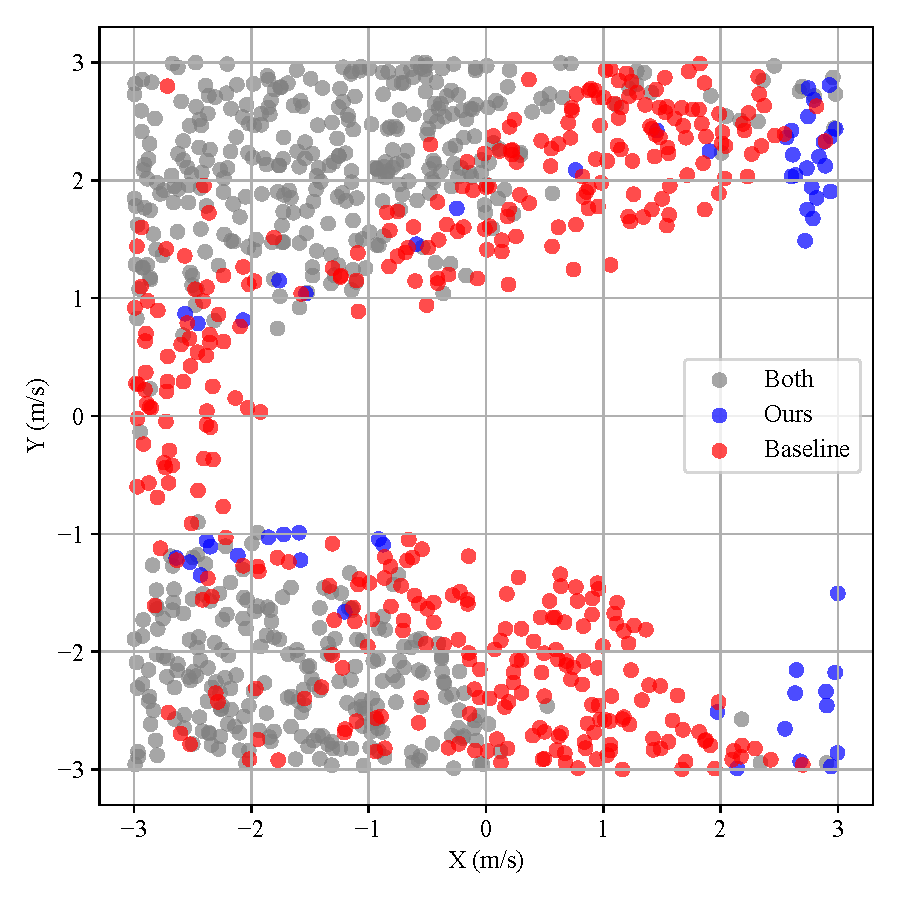
\includegraphics[width=0.8\linewidth]{fig/push.pdf}
    \caption{\textbf{Fall resistant visualization with external push.} `Both' represents cases where both ours and baseline fall. `Ours' and `Baseline' represent cases where each falls but the other survives.}
    \label{fig:push}
\end{figure}

\subsection{Evaluation on Real World}
To test the effectiveness of policy deployment in the real world, we designed a variety of challenging scenarios as shown in Figure~\ref{fig:realworld}.
We deployed the policy for training 2000 iterations on the UniTree A1 robot, with the PD controller's parameters set to $Kp=40.0$ and $Kd=1.0$.
The robot was instructed to walk forward with a command of \([1, 0, 0] \, \text{m/s}\) in five scenarios.
We measured the tracking errors \(||v_{x,y} - v^{target}_{x,y}||^2\) as the performance metric to evaluate the robot's ability to track the linear velocity command, where the body velocity \(v_{x,y}\) is collected by the robot's IMU.
The results in Figure~\ref{fig:realworld_bar} show that our method has a lower tracking error in five scenarios compared to the baseline.

\begin{figure}[h]
    \centering
    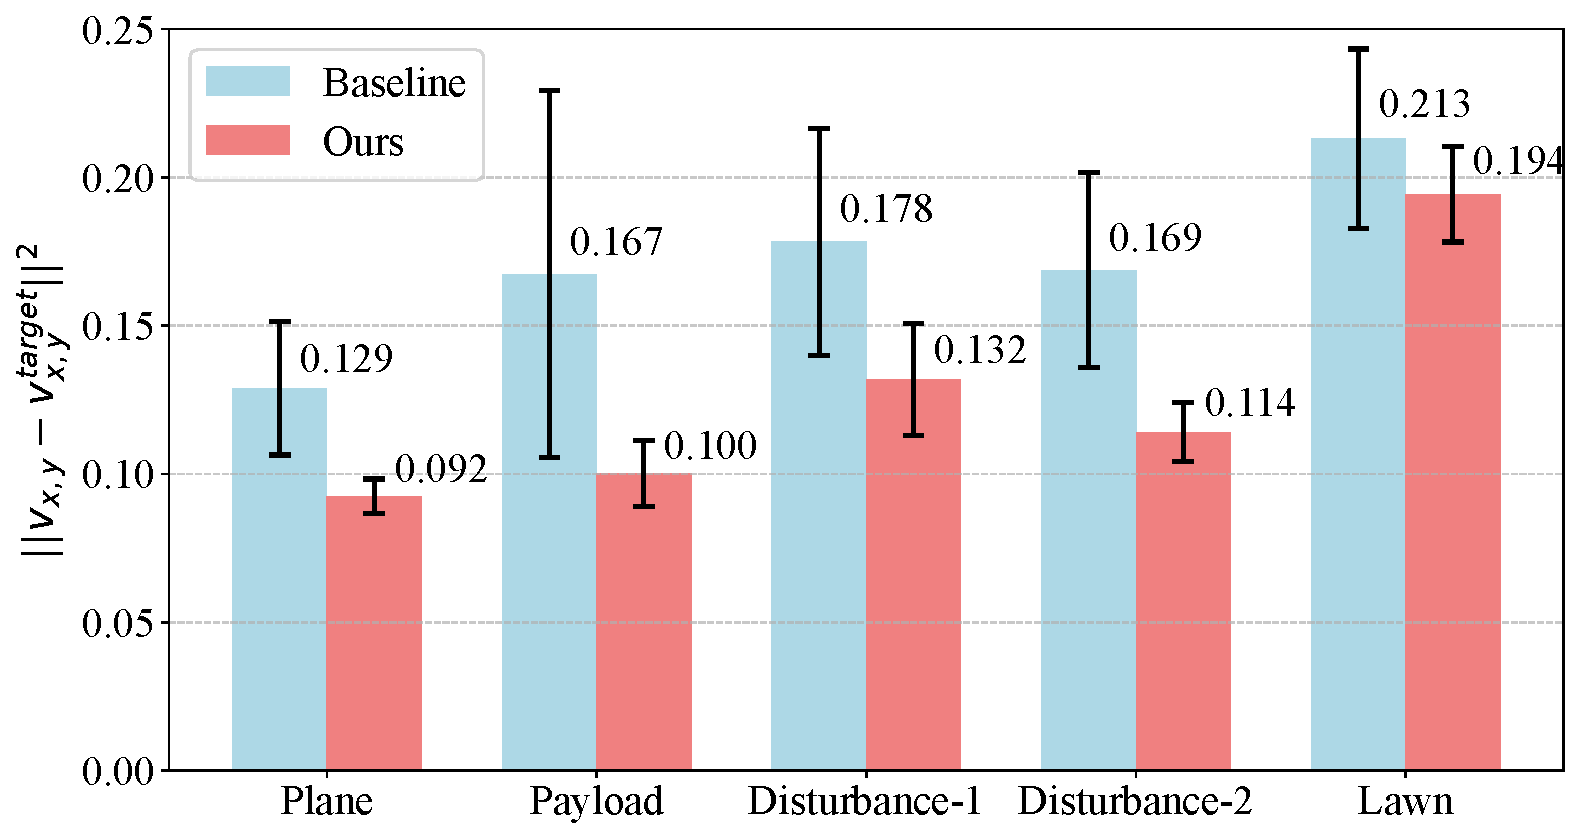
\includegraphics[width=1\linewidth]{fig/realworld_bar.pdf}
    \caption{\textbf{Comparison of command tracking performance in real-world scenarios.} The results are averaged over ten trials. Error bars represent standard error. A lower tracking error indicates better deployed performance.}
    \label{fig:realworld_bar}
\end{figure}


\subsection{Implementation Details}
\paragraph{Reward Design}
The design of reward functions follows previous research\cite{nahrendra2023dreamwaq} and is shown in Table~\ref{tab:reward}.
\begin{table}[h]
% \footnotesize
% \tabcolsep=2pt
    \centering
    \caption{Reward functions.}
    \scalebox{1.05}{
    \begin{tabular}{lll}
    \toprule
    Reward & Equation $\left(r_i\right)$ & Weight $\left(w_i\right)$ \\
    \midrule
    \makecell[l]{Linear velocity\\tracking} & $\exp \left\{- \frac{\|\mathbf{v}_{x y}^{\text{cmd}}-\mathbf{v}_{x y}\|_2^2}{0.25}  \right\}$ & 1.0 \\
    \makecell[l]{Angular velocity\\tracking} & $\exp \left\{- \frac{\left(\omega_{\text {yaw}}^{\text{cmd}}-\omega_{\text{yaw}}\right)^2}{0.25} \right\}$ & 0.5 \\
    Lin. velocity $(z)$ & $v_z^2$ & -2.0 \\
    Ang. velocity $(x y)$ & $\|\boldsymbol{\omega}_{x y}\|_2^2$ & -0.05 \\
    Orientation & $\|\mathbf{g}\|_2^2$ & -0.2 \\
    Joint accelerations & $\|\ddot{\boldsymbol{\theta}}\|^2$ & $-2.5 \times 10^{-7}$ \\
    Joint power & $|\boldsymbol{\tau} \| \dot{\boldsymbol{\theta}}|^{T}$ & $-2 \times 10^{-5}$ \\
    Body height & $\left(h^{\text {target}}-h\right)^2$ & -1.0 \\
    Foot clearance & $\sum_{i=0}^{3}\left(p_{z}^{\text {target}}-p_{z}^{i}\right)^2 \cdot v_{xy}^{i}$ & -0.01 \\
    Action rate & $\|\mathbf{a}_t-\mathbf{a}_{t-1}\|_2^2$ & -0.01 \\
    Smoothness & $\|\mathbf{a}_t-2 \mathbf{a}_{t-1}+\mathbf{a}_{t-2}\|_2^2$ & -0.01 \\
    \bottomrule
    \end{tabular}
    }
    \label{tab:reward}
\end{table}

Where $h^{\text{target}}$ is the desired base height corresponding to ground, $p_z^{\text{target}}$ and $p_z^i$ are the desired feet position and real feet position in the z-axis of robots' frame and $v_{xy}^i$ is the feet velocity in xy-plane of robot's frame.

\paragraph{Dynamics Randomization} We randomize the mass of the robot body and links, the center of mass (CoM) of the robot, the payload applied to the body of the robot, the ground friction and restitution coefficients, the motor strength, the joint-level PD gains, the system delay, the external force, and the initial joint positions during policy Learning with imagined transition. The randomization ranges for each parameter are detailed in Table~\ref{tab:random}.

\begin{table}[h]
% \footnotesize
    \centering
    \caption{Domain Randomization.}
    \scalebox{1.05}{
    \begin{tabular}{lll}
    \toprule 
    Parameters & Range & Unit \\
    \midrule
    CoM & {$[-0.05,0.05]$} & $\mathrm{m}$ \\
    Payload Mass & {$[-1,2]$} & $\mathrm{Kg}$ \\
    Ground Friction & {$[0.2,1.25]$} & - \\
    Motor Strength & {$[0.9,1.1] \times$ motor torque } & $\mathrm{Nm}$ \\
    Joint $K_p$ & {$[0.9,1.1] \times$ 40.0} & Nm/rad \\
    Joint $K_d$ & {$[0.9,1.1] \times$ 1.0} & Nms/rad \\
    Initial Joint Positions & {$[0.5,1.5] \times$ nominal value } & $\mathrm{rad}$ \\
    System Delay & {$[0,15]$ } & $\mathrm{ms}$ \\
    External Force & {$[-30, 30]$} & $\mathrm{N}$ \\
    \bottomrule
    \end{tabular}
    }
    \label{tab:random}
\end{table}

\paragraph{Training Curriculum}
To facilitate robot learning, we adopt a terrain curriculum and command curriculum inspired by the approaches of \cite{rudin2022learning}, \cite{wu2023learning}, and \cite{long2024him}. 
Specifically, we construct a height field map comprising 200 distinct terrains organized in a $20 \times 10$ grid. Within each row, terrains are arranged in increasing order of difficulty, and each grid cell measures $10 \times 10 \, m^{2}$. 
Initially, robots are placed on the simplest terrain types. As the robot's performance improves, the terrain difficulty level increases once the robot achieves at least 80\% of the linear tracking reward. Conversely, the difficulty decreases if the robot cannot traverse half of the terrain within a single episode.
For terrains involving stairs or discrete obstacles, we sample longitudinal and lateral linear velocity commands from the range $[-1.0, 1.0]$ m/s and the horizontal angular velocity from $[-2.0, 2.0]$ rad/s. For slopes and rough terrains, the range of longitudinal linear velocity is extended to $[-3.0, 3.0]$ m/s, and the range for horizontal angular velocity is expanded to $[-3.0, 3.0]$ rad/s. All commands are sampled independently for each robot from the specified ranges, with sampling occurring every 25-time steps.